%%% DOCUMENT BEGIN

\documentclass{article}

\usepackage[utf8]{inputenc}

\usepackage{geometry}
\geometry{a4paper}



%%% PACKAGES
\usepackage{lastpage}
\usepackage{graphicx}
\usepackage{booktabs} % for much better looking tables
\usepackage{array} % for better arrays (eg matrices) in maths
\usepackage{paralist} % very flexible & customisable lists (eg. enumerate/itemize, etc.)
\usepackage{verbatim} % adds environment for commenting out blocks of text & for better verbatim
\usepackage{subfig} % make it possible to include more than one captioned figure/table in a single float
\usepackage{float}


%%% HEADERS & FOOTERS
\usepackage{fancyhdr} % This should be set AFTER setting up the page geometry
\pagestyle{fancy} % options: empty , plain , fancy
\renewcommand{\headrulewidth}{0pt} % customise the layout...
\lhead{}\chead{}\rhead{}
\lfoot{}\cfoot{\thepage}\rfoot{}

%%% SECTION TITLE APPEARANCE
\usepackage{sectsty}
\allsectionsfont{\sffamily\mdseries\upshape}

%%% ToC (table of contents) APPEARANCE
\usepackage[nottoc,notlof,notlot]{tocbibind} % Put the bibliography in the ToC
\usepackage[titles,subfigure]{tocloft} % Alter the style of the Table of Contents
\renewcommand{\cftsecfont}{\rmfamily\mdseries\upshape}
\renewcommand{\cftsecpagefont}{\rmfamily\mdseries\upshape} % No bold!


%%% END Article customizations



\widowpenalties 1 10000

%%%%%%%%%%%%%%%%%%%%%%%%%
%%%          Fill in the title details                      %%%

\def \thetitle {INF-1400-Object Oriented Programming}
\def \thesubtitle {Mandatory assignment 3}
\def \theauthor {Helge Hoff \& Øystein Tveito}

%%%%%%%%%%%%%%%%%%%%%%%%%

%\pagestyle{fancy}
\pagestyle{fancyplain} % options: empty , plain , fancy
\renewcommand{\headrulewidth}{1pt} % customise the layout...
\renewcommand{\footrulewidth}{0pt}
\lhead{\fancyplain{}{\thetitle{} -- \thesubtitle{}}}\chead{}\rhead{\fancyplain{}{\theauthor{}}}
\lfoot{}\cfoot{Page {\thepage} of \pageref{LastPage}}\rfoot{}

\begin{document}

%%% TITLE PAGE

\begin{titlepage}
\begin{center}

\textsc{\\[3.5cm] \huge University of Tromsø}\\[1.5cm]

\textsc{\LARGE \thetitle}\\[0.5cm]

\textsc{\Large \thesubtitle}\\[1.5cm]

\LARGE{\theauthor} \\[0.5cm] \large{Department of Computer Science}

\vfill
{\large \today}

\end{center}
\thispagestyle{empty}
\end{titlepage}

\newpage{}


%%% TABLE OF CONTENTS

\tableofcontents


\newpage{}

%%% DOCUMENT BODY

%%% Set counter to 1
%\setcounter{page}{1}
\section{Introduction}
\paragraph{}
For this project a clone of the arcade game Mayhem will be implemented. There is two authors on this project, so the workload will be shared between.
\subsection{Technical Background}
\subsubsection{Mayhem} 
\paragraph{}
A classic arcade game with two (or more) spaceships fight each other. 
\section{Design}
\paragraph{}
This game is a two player game sharing one screen and keyboard. Each player have a set of keys associated with him, making him able to navigate and shoot his spaceship. Each spaceship starts at a spawn point which is a platform not affected by gravity. On the platform, the player can refuel and restock bullets. The platform a player spawn on is private, and can not be used by other players. 
\paragraph{}
In the middle of the screen there is a black hole. The black hole has gravity, pulling every player towards it. It also pulls laser bullets, because, as we know, not even light can escape the awesome power of a black hole. This is done instead of having gravity pointing downwards. The scene is set in space, so there is no up and down. When getting close to the black hole, an object will start to spin clockwise towards around the hole, while pulling it towards the center. 
\paragraph{}

\section{Implementation}
\paragraph{}
The game is written in python, with pygame as it's most significant building block. All classes are split into separate files for a better overview of the game. All visible objects are children of the pygame class Sprite.

\begin{figure}[hbtp]
\caption{Class diagram}
\centering
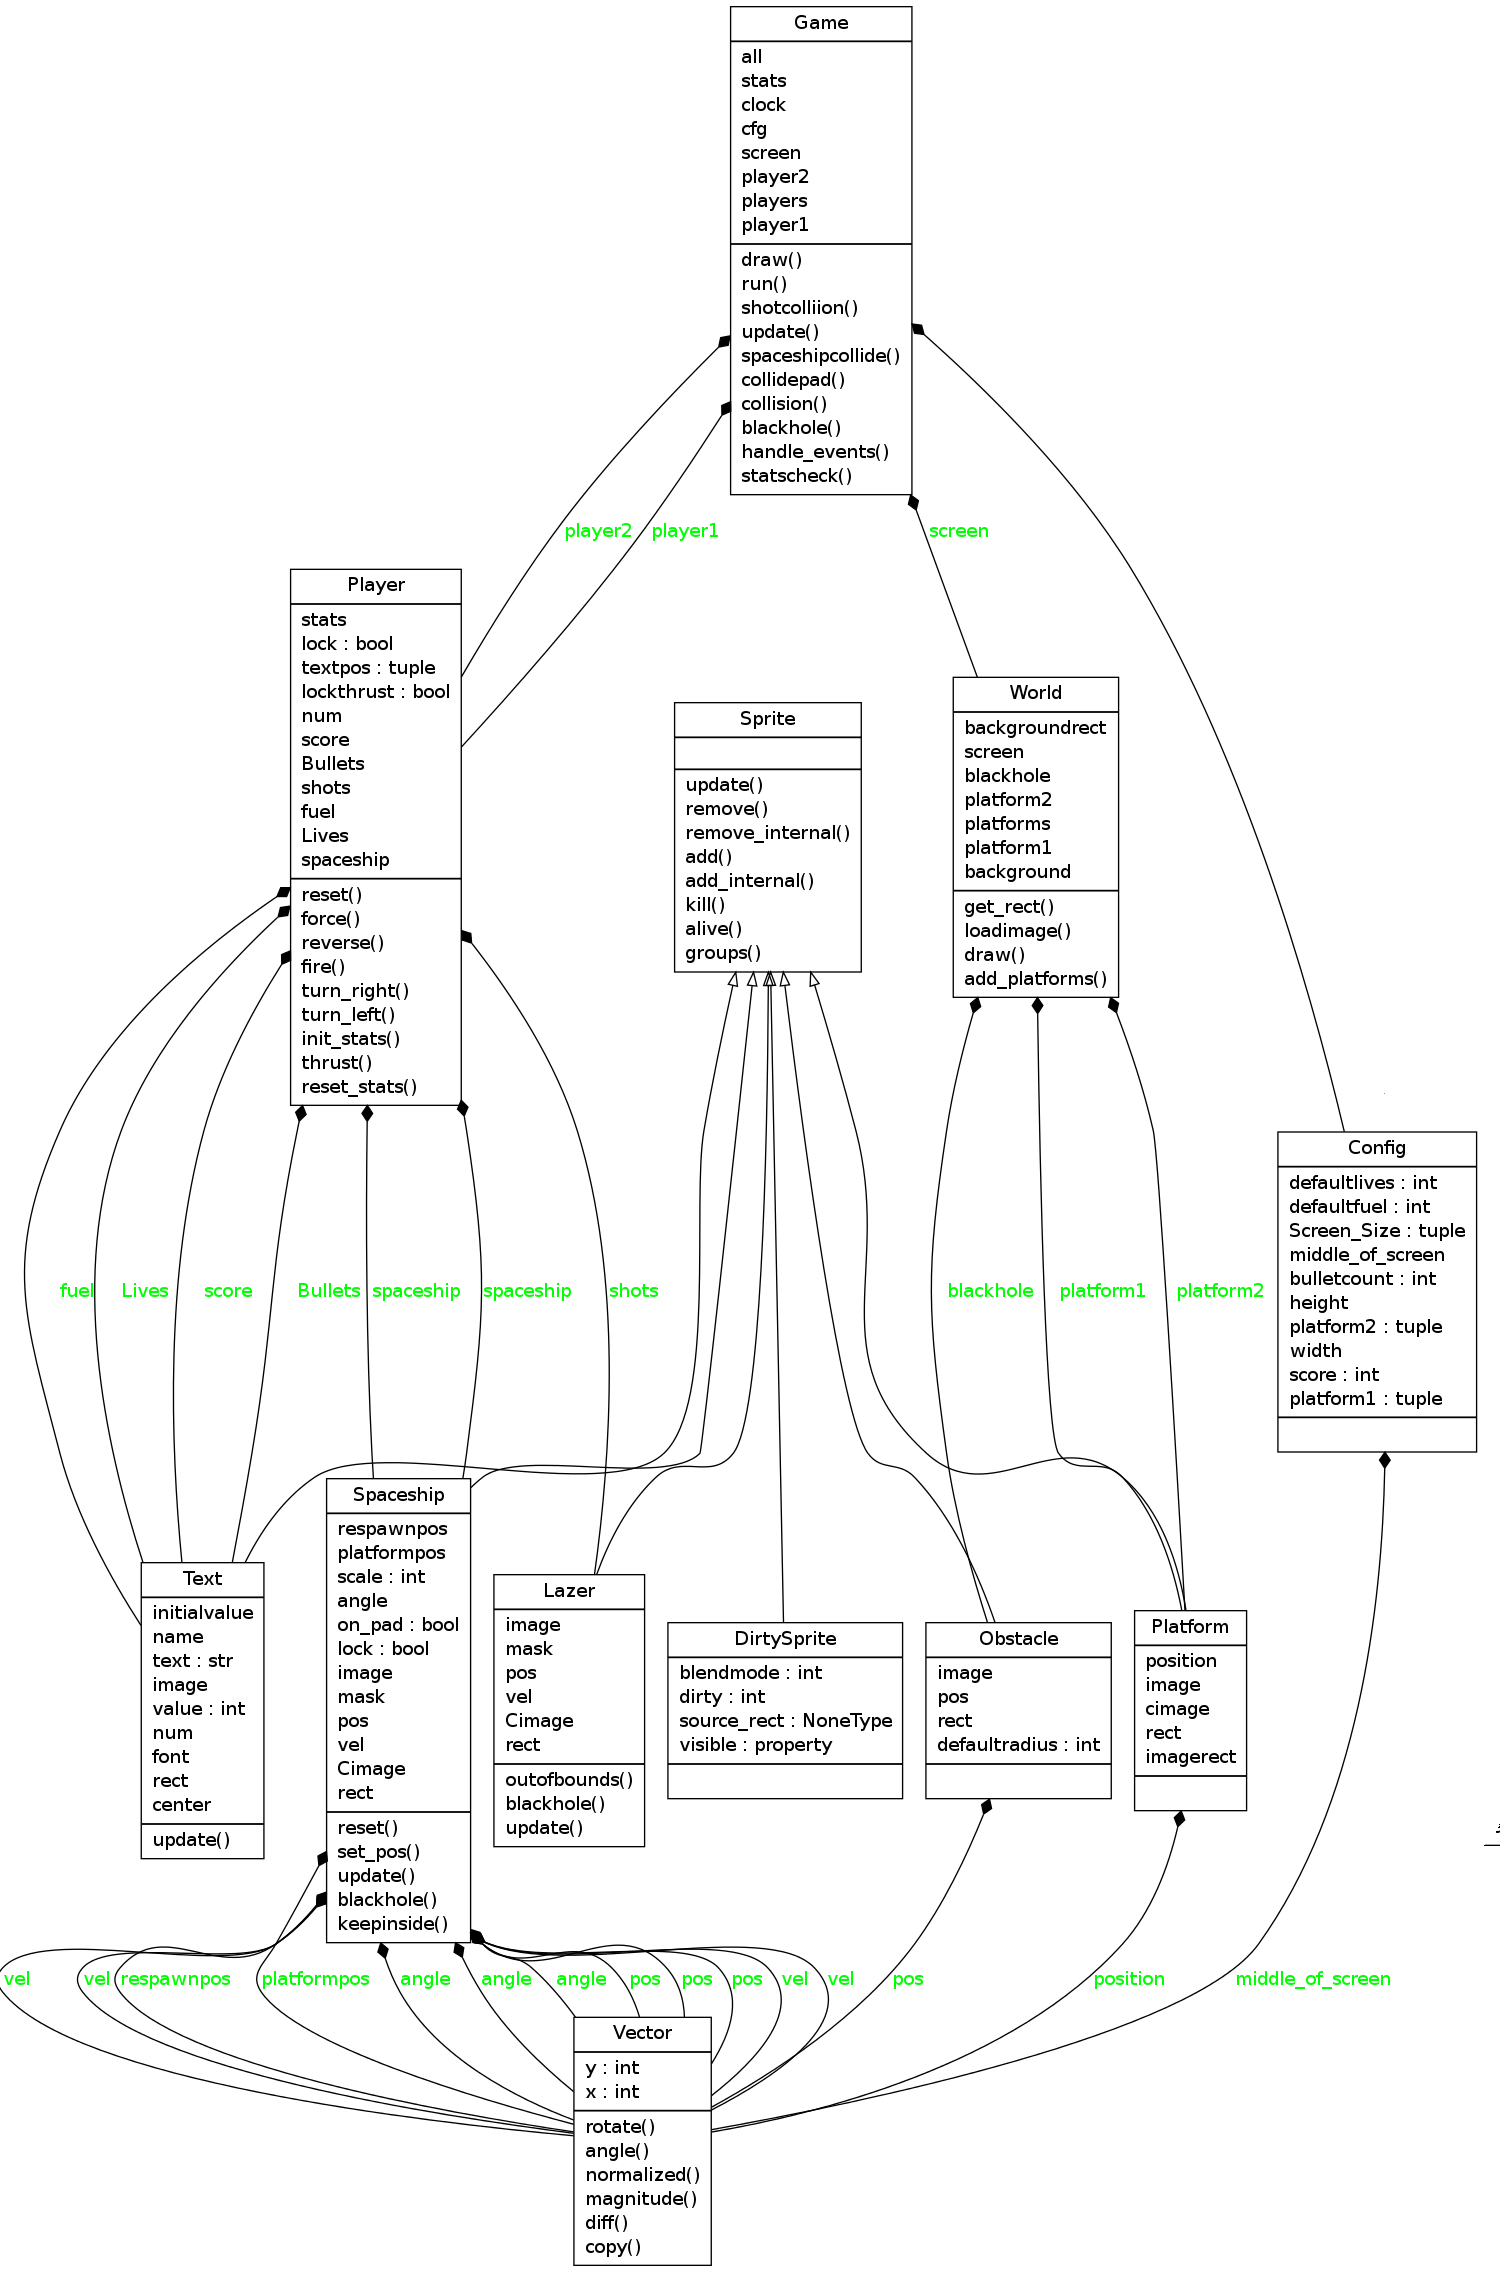
\includegraphics[scale=0.3]{classdiagram.png}
\end{figure}
\newpage

\subsection{World}
\paragraph{}
The World class contains the screen on which all of the games objects are to be drawn. It also contains the backround image represented as a pygame surface type, the black hole, and the two platforms where the spaceships are spawned. The platforms is of type pygame sprite object aswell as the black hole represented in the middle of the screen where the spachips disappear into when drawing to close.
\subsection{Text}
\paragraph{}
The text is as the requirements specified of type pygame sprite, and each status parameter of the spaceships is one objects which is put in a pygame sprite group. the text object has an update method which renders the text for later to be drawn. The different status attribute of the spaceships can be altered by changing the different objects values, value is an attribute of the text class.
\subsection{Collision}
\subsubsection{Spaceships}
\paragraph{}
Collision between the two spaceships is handled by using the pygame sprite mask collision method which has two sprites as input. Then the two spaceship sprites are sent in as arguments to the mask collide function. Then if collision they each looses lives.
\subsubsection{Bullets}
\paragraph{}
The bullets for the specific spaceship is in its own group which fasilitates the collision detection. Here the mask collide method is also used, and to check every bullet from one spaceship towards the other spaceship is done by getting a list of sprites that the sprite group contains. Then iterating through it and checking every bullet up against the spaceship. To get a list of the sprites in a group is simply done by setting a list equal to the specific group.
\subsubsection{On pad detection}
\subsection{Player}
\paragraph{}
\subsection{Game}
\subsection{Spaceship}

 



\section{Discussion}
\paragraph{}
This section starts with a list of requirements and an explanation on whether or not this implementation has successfully implemented this:
\begin{itemize}
	\item Two spaceships with four controls: rotate left, rotate right, thrust, fire.
	\begin{itemize}
		\item All the controls are implemented with the addition of backwards thrust. The backwards thrust is added to make it easier to avoid the black hole, and in the same time be able to shoot against your opponent.
	\end{itemize}
	\item Minimum one obstacle in the game world. This can be as simple as a single rectangle in the middle of the screen.
	\begin{itemize}
		\item A black hole has been added as an obstacle in the middle of the world.
	\end{itemize}
	\item Spaceship can crash with walls/obstacles/other spaceship.
	\begin{itemize}
		\item The spaceships will be absorbed by the black hole. In the event of a crash with an other spaceship, the spaceship with the least amount of health will be destroyed.
	\end{itemize}
	\item Gravity acts on spaceships (the original has no gravity acting on the
	bullets, but you can choose what works best).
	\begin{itemize}
		\item There is no gravity pulling downwards because this is in space. The black hole stands for the gravity, pulling everything towards it and in a spiral.
	\end{itemize}
	\item Each player has a score that is displayed on the screen. A player's score increases when he shoots down the opponent. A player's score decreases if he crashes.
	\begin{itemize}
		\item A score is implemented and shown on screen. The score increases when a shot from that ship hits the opponent. On destruction the score will be reset to zero.
	\end{itemize}
	\item  Each spaceship has a limited amount of fuel. To refuel, it must land on one of two landing pads. Alternatively, you can put a "fuel barrel" at a random position that is collected by the first spaceship reaching it.
	\begin{itemize}
		\item Each spaceship has its own fuelling pad that recharges its fuel and bullets. The pad is unique to the spaceship, so a player can only land on his own pad.
	\end{itemize}
	\item Scrolling window, as seen on the video, is NOT a requirement.
	\begin{itemize}
		\item Not implemented.
	\end{itemize}
	\item The implementation must consist of a minimum of two files. One of these shall be a config.py file containing global configuration constants, such as screen size, amount of gravity, amount of starting fuel.
	\begin{itemize}
		\item The config file is implemented and holds some variables that govern screen size and some initial values.
	\end{itemize}
	\item The main loop must have timing so that the game is playable on different computers.
	\begin{itemize}
		\item The game loop is controlled by the pygame clock. This is set to 60 ticks each second, so as long as the computer can handle 60 FPS (any fairly modern computer can) the game will feel the same. If the computer is to slow for this, it will be slower. This is done to not make the spaceship jump long distances for each frame.
	\end{itemize}
	\item The game shall be started using Python's if \_\_name\_\_ == '\_\_main\_\_': idiom. Inside the if test, a single line shall be instantiate the game object. All other code, except the game configuration constants, shall be inside the classes. This will simplify profiling and documentation generation.
	\begin{itemize}
		\item The first exception from this rule is that the main function is in a file of its own. To make the game run, pygame need to be initiated in every file expecting to have anything with pygame. For this reason, the first line in main is initialization of pygame. The second exception is that the game class do not start the game by it self. This is done on purpose, so the caller can initiate the object, and chose when to start it. Giving more control to the user is a informed choice, and the authors stand by it.
	\end{itemize}
	\item All visible objects shall subclass the pygame.sprite.Sprite class. The sprites shall be put into groups using pygame.sprite.Group. Then updating and drawing shall be performed using Group.update and Group.draw. 
	\begin{itemize}
		\item Every visible object is a subclass of sprite, and every object is updated and drawn using the Sprite functionality.
	\end{itemize}
	\item All modules (files), classes and methods shall contain docstrings. If you are working in a team, the module docstring at the top of the file shall contain the name of both authors. When you are done programming, html documentation shall be generated using pydoc -w command.
	\begin{itemize}
		\item This requirement is met.
	\end{itemize}
	\item The last task is to profile the code using cProfiler. Take a screenshot of the result and include it in the report. Giva a short summary of the sesult and discuss where you would focus to imporve the performance of the implementation.
	\begin{itemize}
		\item 
	\end{itemize}
\end{itemize}

\section{Conclusion}
\paragraph{}



\begin{thebibliography}{9}

\bibitem{boids}
  wikipedia.org,
  \emph{Boids}:
  http://en.wikipedia.org/w/index.php?title=Boids\&oldid=580365466 
  [Online; accessed 26-02-2013]
  
\bibitem{leap}
  wikipedia.org,
  \emph{Leap}:
  http://en.wikipedia.org/w/index.php?title=Leap\_Motion\&oldid=592637003
  [Online; accessed 03-03-2013]
  

\end{thebibliography}



\end{document}
